\documentclass[preprintnumbers,amsmath,amssymb,onecolumn,12pt]{revtex4}
\usepackage{graphicx}% Include figure files
\usepackage{dcolumn}% Align table columns on decimal point
\usepackage{bm}% bold math
\usepackage{natbib}
\usepackage{physics}
\usepackage[caption=false]{subfig}

\def\sgn{\mathop{\rm sgn}}

\begin{document}

\vspace{0.2in}
{\Large \hspace{1.6in}\textsc{Supplementary Material} }\\
\
\title{Mechanical Detection of Dipole-Dipole Interactions \\between Electronic Spins in a Solid}

\author{C. Pellet-Mary, P. Huillery, M. Perdriat, G. H\'etet} 


\affiliation{$^1$
Laboratoire de Physique de l'Ecole normale sup\'erieure, ENS, Universit\'e PSL, CNRS, Sorbonne Universit\'e, Universit\'e Paris-Diderot, Sorbonne Paris Cit\'e, Paris, France.
}

\begin{abstract}
\end{abstract}

\maketitle

\tableofcontents

\newpage

\section{NV$^-$ center Theory}
\subsection{NV spin Hamiltonian}
The NV spin Hamiltonian in its fundamental level can be written as :
\begin{equation*}
  \hat{\mathcal{H}}_s=D S_z^2 + \gamma_e \textbf{B}\cdot\hat{\textbf{S}},
  \end{equation*} 
Where $D = (2\pi) 2.87$ GHz is the crystal field splitting originating from a spin-spin interaction, and $\gamma_e = 28 $GHz/T is the electron gyromagnetic ratio. We neglected contributions of the strain and local electric field since we are working with magnetic fields of the order of 100G, as well as the hyper-fine interaction with $^{14}$N since we are working with ensembles with a typical inhomogeneous broadening $\frac{1}{T_2^*} \approx (2\pi) 5$ MHz.

The \textbf{z} axis of the $S_z$ operator here is the axis formed by the nitrogen atom and the vacancy, hence why we do have different energy transitions for different NV orientations, depending on the projection of the magnetic field on the NV axis.

\subsection{Diamond crystalline axes and degeneracy conditions}
\begin{figure}[!ht]
  \centering \scalebox{0.45}{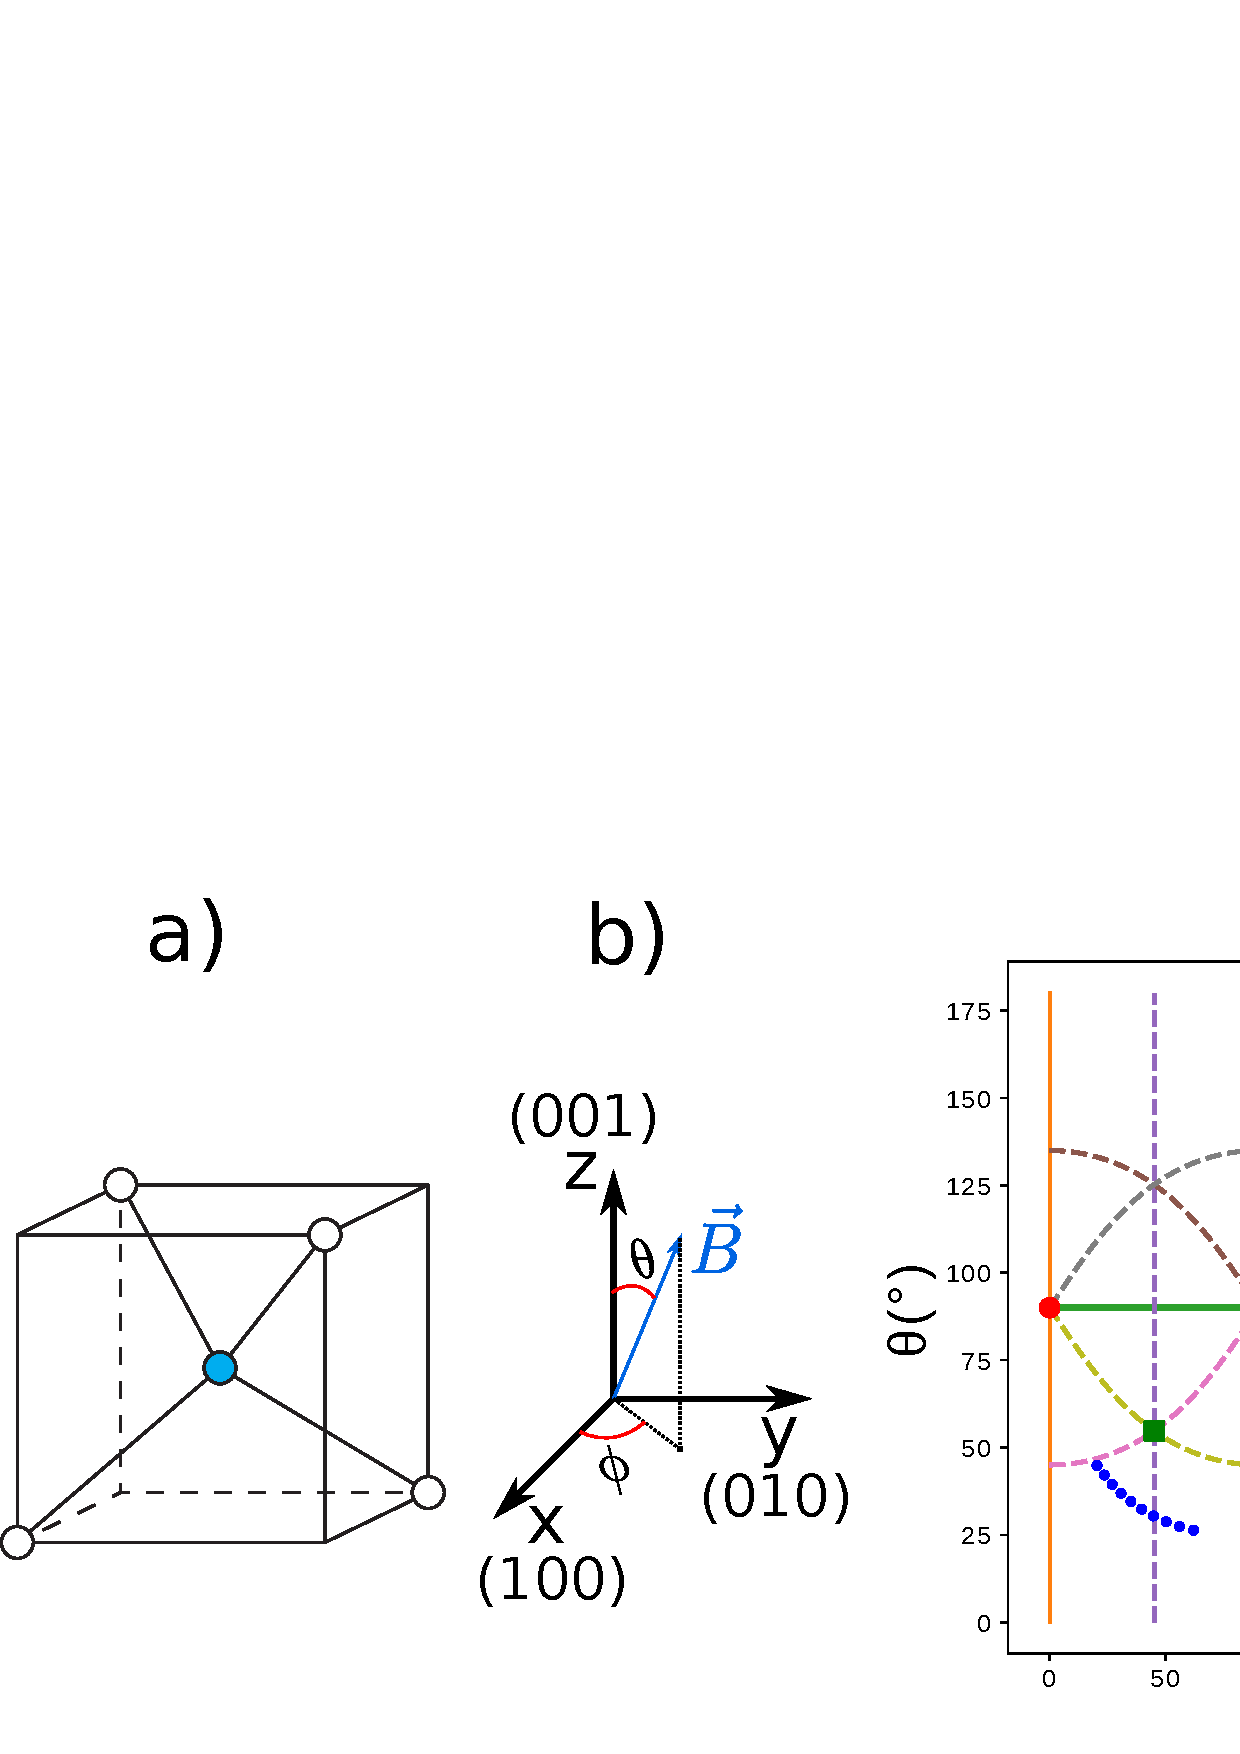
\includegraphics{SI_Cristallo}}
  \caption{a) Representation of the four crystalline axes of the diamond b) Representation of the magnetic field in the diamond crystalline basis c) Representation in the $(\theta , \phi)$ basis of the crystalline planes ([110]$_\perp$ family of planes in dashed lines, [100]$_\perp$ in plain lines), [100] direction as a red circles, [111] direction as a green squares and the path of the magnetic field in the experiment of Fig. 3 of the main text in blue dots.}
	\label{cristallo}
\end{figure}
There are four possible crystalline axis for the NV centers (so-called "classes" of NV) which are depicted in Fig. \ref{cristallo} b) and correspond to the crystalline directions [$111$], [$1\bar 1 \bar 1$], [$\bar 1 1 \bar 1$] and [$\bar 1 \bar 1 1$]. 

The magnetic field is represented in the diamond basis in Fig. \ref{cristallo} a) where the usual polar and azimuthal angles $\theta$ and $\phi$ are defined with respect to the \textbf{z} ([$001$]) direction.

For some orientations of the magnetic field, the projection of the magnetic field on two or more NV axes will be identical, and therefore the energy level of the corresponding classes will be the same. These degeneracies are represented on fig \ref{cristallo} c), where the dashed lines are the locus of the crystalline planes orthogonal to the [110] directions (6 planes in total). When the magnetic field belongs to these plane, we observe a degeneracy between two classes of NV, as can be seen in the Fig. 4 of the main paper.

The plain lines are the locus of the planes orthogonal to the [100] directions (3 planes total). When the magnetic field is in these planes, every class is at resonance with another class, as can be seen in Fig. X.

The red circles correspond to the [100] directions, for which the four classes of NV or at degeneracy, and the green squares to the [111] direction where one class is aligned with the magnetic field, and the three other are at degeneracy.

Finally the blue dots correspond to the path followed by the magnetic field in the experiment presented in Fig 4. of the main text, where we can see a degeneracy plane of the [110]$_\perp$ family being crossed.

\section{Experimental details}

\subsection{Experimental setup}

\begin{figure}[!ht]
  \centering \scalebox{0.3}{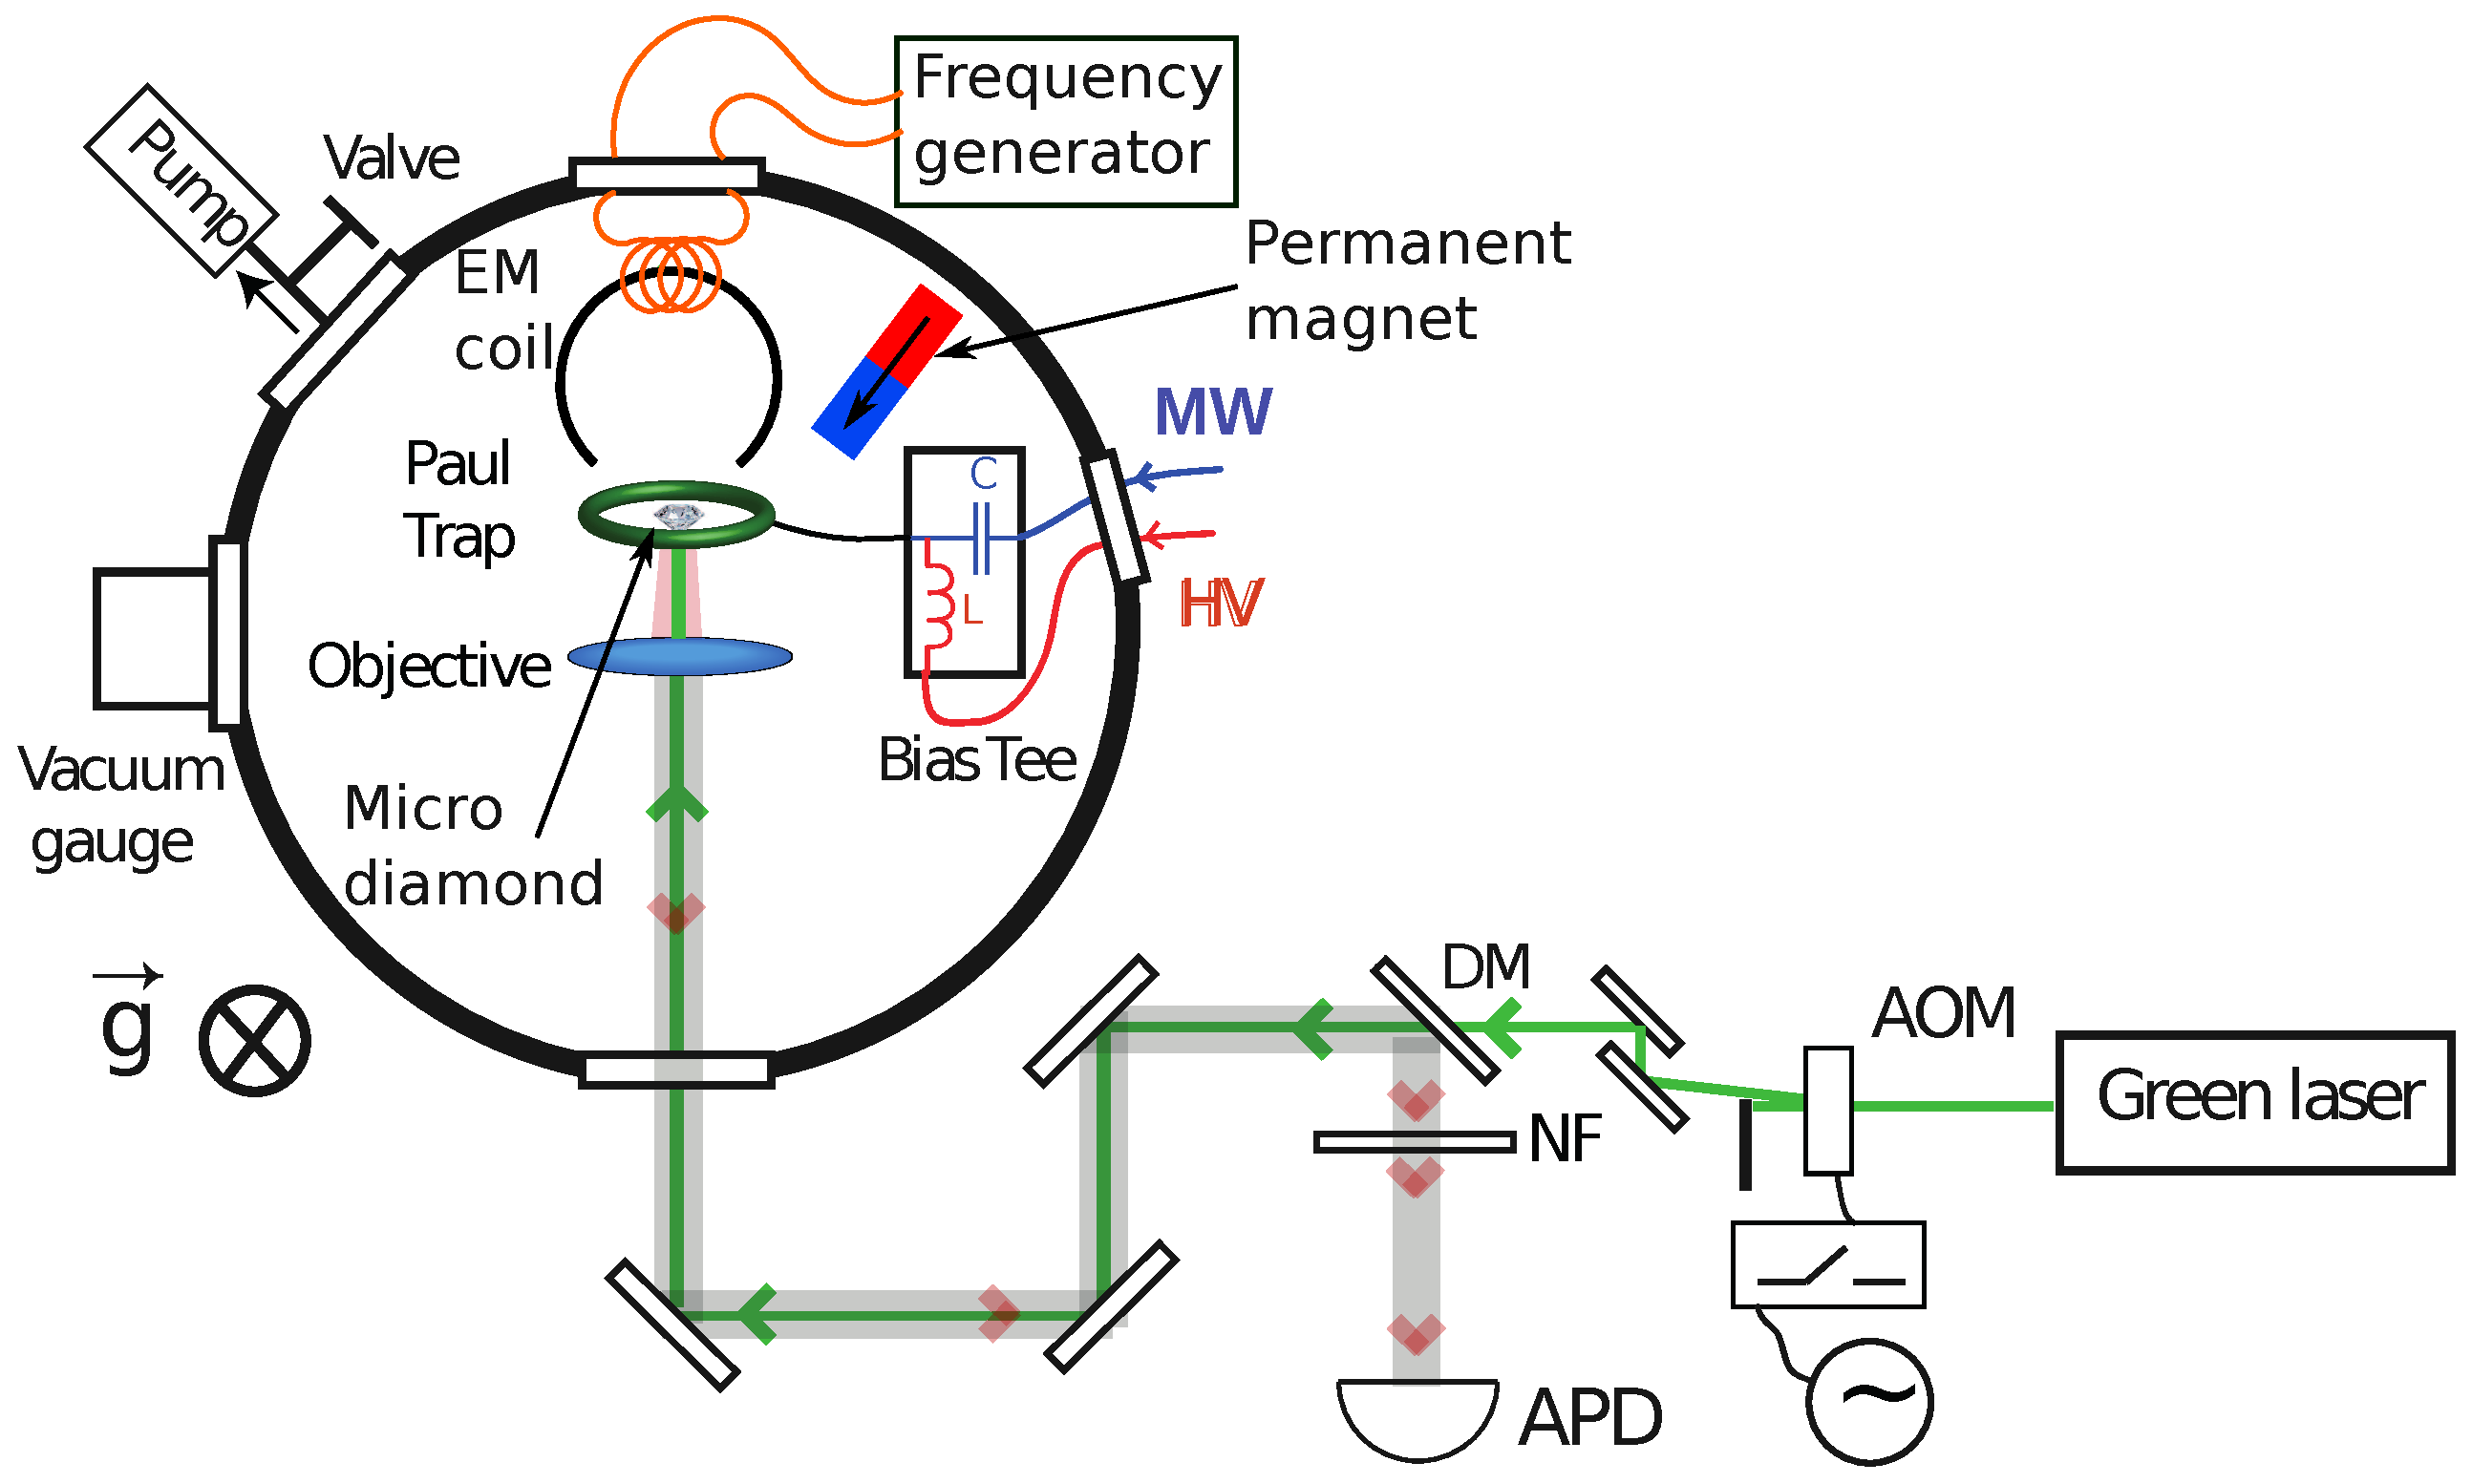
\includegraphics{setup}}
  \caption{Illustration of the experimental setup}
	\label{Optics}
\end{figure}

The experimental setup illustrated in Fig.\ref{Optics} is very similar to the one used in \citep{DelordPRL} with the addition of a permanent magnet and an electromagnetic (EM) coil in order to perform magnetic field scans. The diamond sample is typically illuminated with 1mW of 532 nm laser light, focused by a NA = 0.5 objective. An acousto-optic modulator (AOM) is used to switch on and off the 532nm laser and to finely tuned its power. The photo-luminescence (PL) is collected by the objective, separated form the excitation light using a dichroic mirror (DM) and a 532nm notch filter (NF), and detected using a multimode-fibered single-photon avalanche photo-detector (APD) (SPCM-AQRH-15 from Perkin Elmer). Typically, we detect PL photons at a rate of 1 MHz. 

The Paul trap is a pseudo-ring with a diameter of approximately 200 $\mu$m, as can be seen in \citep{DelordPhD}. It acts both as trap through the high voltage (HV) and as a microwave (MW) antenna.

The magnetic field generated by the (homemade) EM coil is controlled by a programmable power supply (Rhode \& Shwartz NGE 103) performing current ramps.

While the levitating setup is located in a vacuum chamber, all the experiments presented in this article are performed at atmospheric pressure.


\subsection{$T_1$ Measurement}
\begin{figure}[!ht]
  \centering \scalebox{1.2}{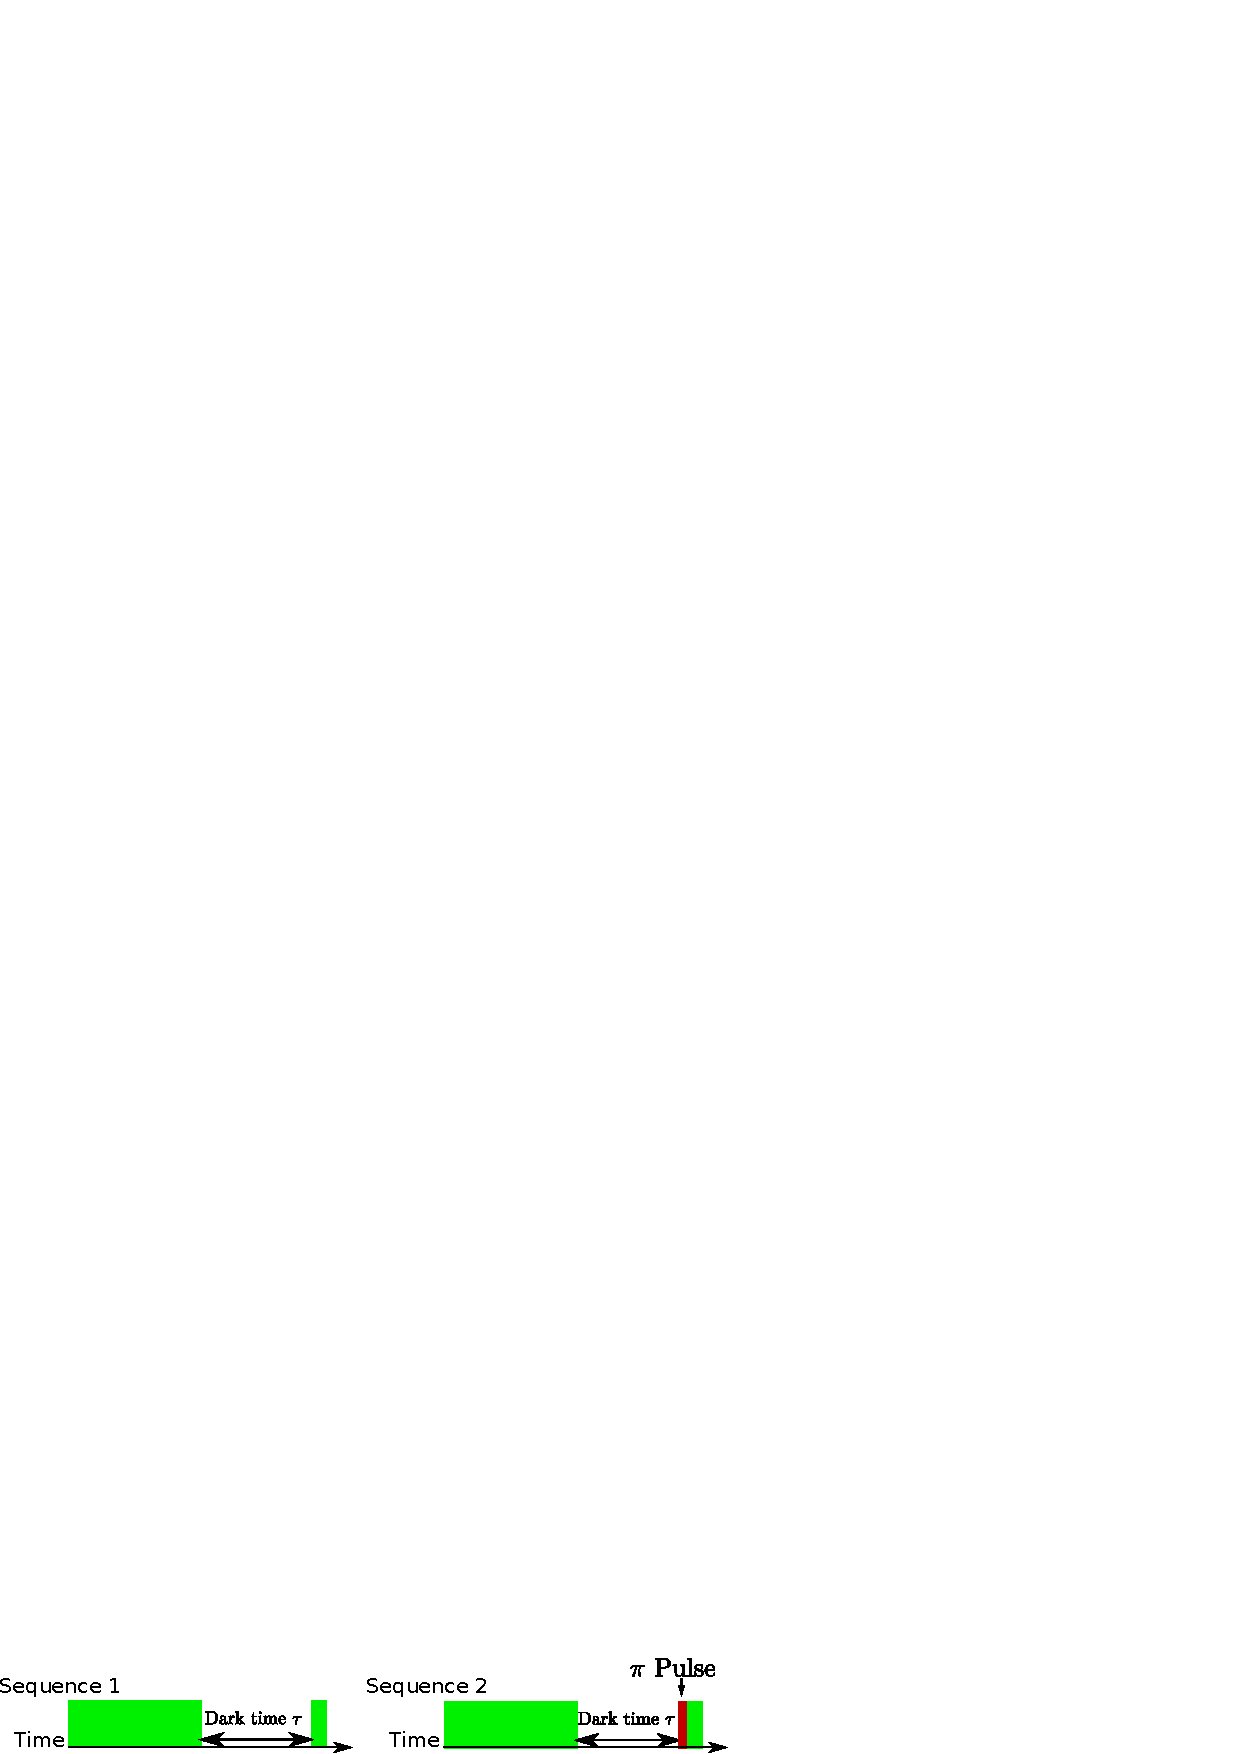
\includegraphics{T1_soustraction_shema}}
  \caption{T$_1$ measurement protocol for a single class in an ensemble of NV centers. Green bars represent laser excitation, red bar represent microwave $\pi$ pulse for the selected class}
	\label{T1_protocol}
\end{figure}
The protocol to measure the spin lifetime of the NV centers, as presented in Fig 2. of the main text, is described in Fig. \ref{T1_protocol} . In the first sequence ($S_1$), the spins are initially polarized in their $m_s=\ket{0}$ state through a 1 ms green laser excitation pulse and then left to evolve in the dark for a variable dark time $\tau$. The spin state is finally read out with a 10 $\mu$s laser pulse, shorter than the polarization time of the spins.

The second sequence ($S_2$) uses the same parameters (polarization time, dark time and readout time) than the first sequence but adds a resonant microwave $\pi$ pulse on a transition of one of the four classes of NV$^-$ right before the readout pulse, exchanging the population of the $m_s=\ket{0}$ state with one of the $m_s=\ket{\pm 1}$ state.

By looking a the subtraction of both signal $S_1-S_2$, we can then measure the spin state population of a single class, and remove unwanted contributions to the photoluminescence, such as charge state transfer in the dark.

\subsection{Magnetic field calibration}

A permanent magnet is placed a few cm away from the diamond sample in order to apply a uniform magnetic field to the NV centers together with an electro-magnet.

To calibrate the magnetic field magnitude $B$, and its orientation $\theta$ with respect to the NV axis, we record Optically Detected Magnetic Resonance (ODMR) spectra.... 



\subsection{Spin-mechanical detection}

The microwave detuning is scanned in 2~MHz steps with a duration of 10 ms per points. During those 10ms, the diamond orientation has enough time to reach its equilibrium position and the spin torque effect can be observed. The average count-rate is about 1 MCounts/s.

\subsection{PL detection}

In these measurements, compared to \cite{DelordNat}, to detect the PL we use another detection channel that is more resilient to motion. We therefore do not need to detect prior to ring down.

\section{Principle of the mechanical detection}

\subsection{Torque sensing with a levitating diamond}

The way we can experimentally measure torques applied on a levitating diamond is by looking at the displacement of equilibrium caused by them. Here is a short model detailing it :

We model the trap as a pure harmonical potential, both for the center of mass and for the rotational degrees of freedom of the diamond (REF qq part), with trapping frequencies $\omega_T \approx 1$ kHz that we can experimentally measure. If we focus on a single rotational degree, we can write the torque generated by the trap as $\Gamma_T^\theta=-K(\theta-\theta_{eq})$, where $K=I \omega_t^2$ is the stiffness of the trap, $I$ being the moment of inertia of the diamond.

The application of an external torque $\Gamma_{\mathrm{ext}}$ on the diamond will therefore shift the angular position at equilibrium in such a way that : 
\begin{align*}
-K(\theta-\theta_{\mathrm{eq}}) + \Gamma_{\mathrm{ext}} &= -K(\theta-\theta_{\mathrm{eq}}') \\
\delta\theta = \theta_{\mathrm{eq}}'-\theta_{\mathrm{eq}} &= \frac{\Gamma_{\mathrm{ext}}}{K}=\frac{\Gamma_{\mathrm{ext}}}{I \omega_t^2}
\end{align*}

In our case, $\Gamma_{\mathrm{ext}}$ is the magnetic torque exerted by the NV$^-$ spins directly on the diamond, such that we can write $\Gamma_{\mathrm{ext}} = N_{NV} \langle \Gamma_{\mathrm{1 spin}} \rangle$  where $\langle \Gamma_{\mathrm{1 spin}} \rangle = \gamma_e \langle\hat{\mathbf S}\rangle \times \mathbf B \approx 10^{-28}$ Nm is the classical magnetic torque applied by one spin (see Section  \ref{Simu}). 

By using the inertia moment formula of a sphere : $I=\frac{2}{5}m r^2$, we can then rewrite the angular displacement as $$ \delta\theta = \frac{\langle\Gamma_{\mathrm{1 spin}}\rangle [NV^-]}{\frac{2}{5}m_Cr^2\omega_T^2} \approx 10^{-3} rad$$ where $[NV^-] \approx 5 \cdot 10^{-6}$ (5 ppm) is the number of NV centers per atoms in the crystal, $m_C \approx 2 \cdot 10^{-26}$ kg is the average weight of a carbon atom (we assume that the bulk of the diamond weight comes from carbon atoms), $r= 7.5$ $\mu$m is the typical radius of our diamonds and $\omega_T = 1$ kHz is the typical value of the trap frequency.

It should be noted that the main uncertainty comes here from the diamond size, which along the other uncertainties can change the expected result by an order of magnitude.

\subsection{Change of torque at the cross-relaxation}

\section{Cross-relaxation detection for another type of degeneracy}

%Faire 2 lignes avec sur la première ligne l'ESR et le trajet sur la carte du champ mag
\begin{figure}[!ht]
  \centering \scalebox{0.32}{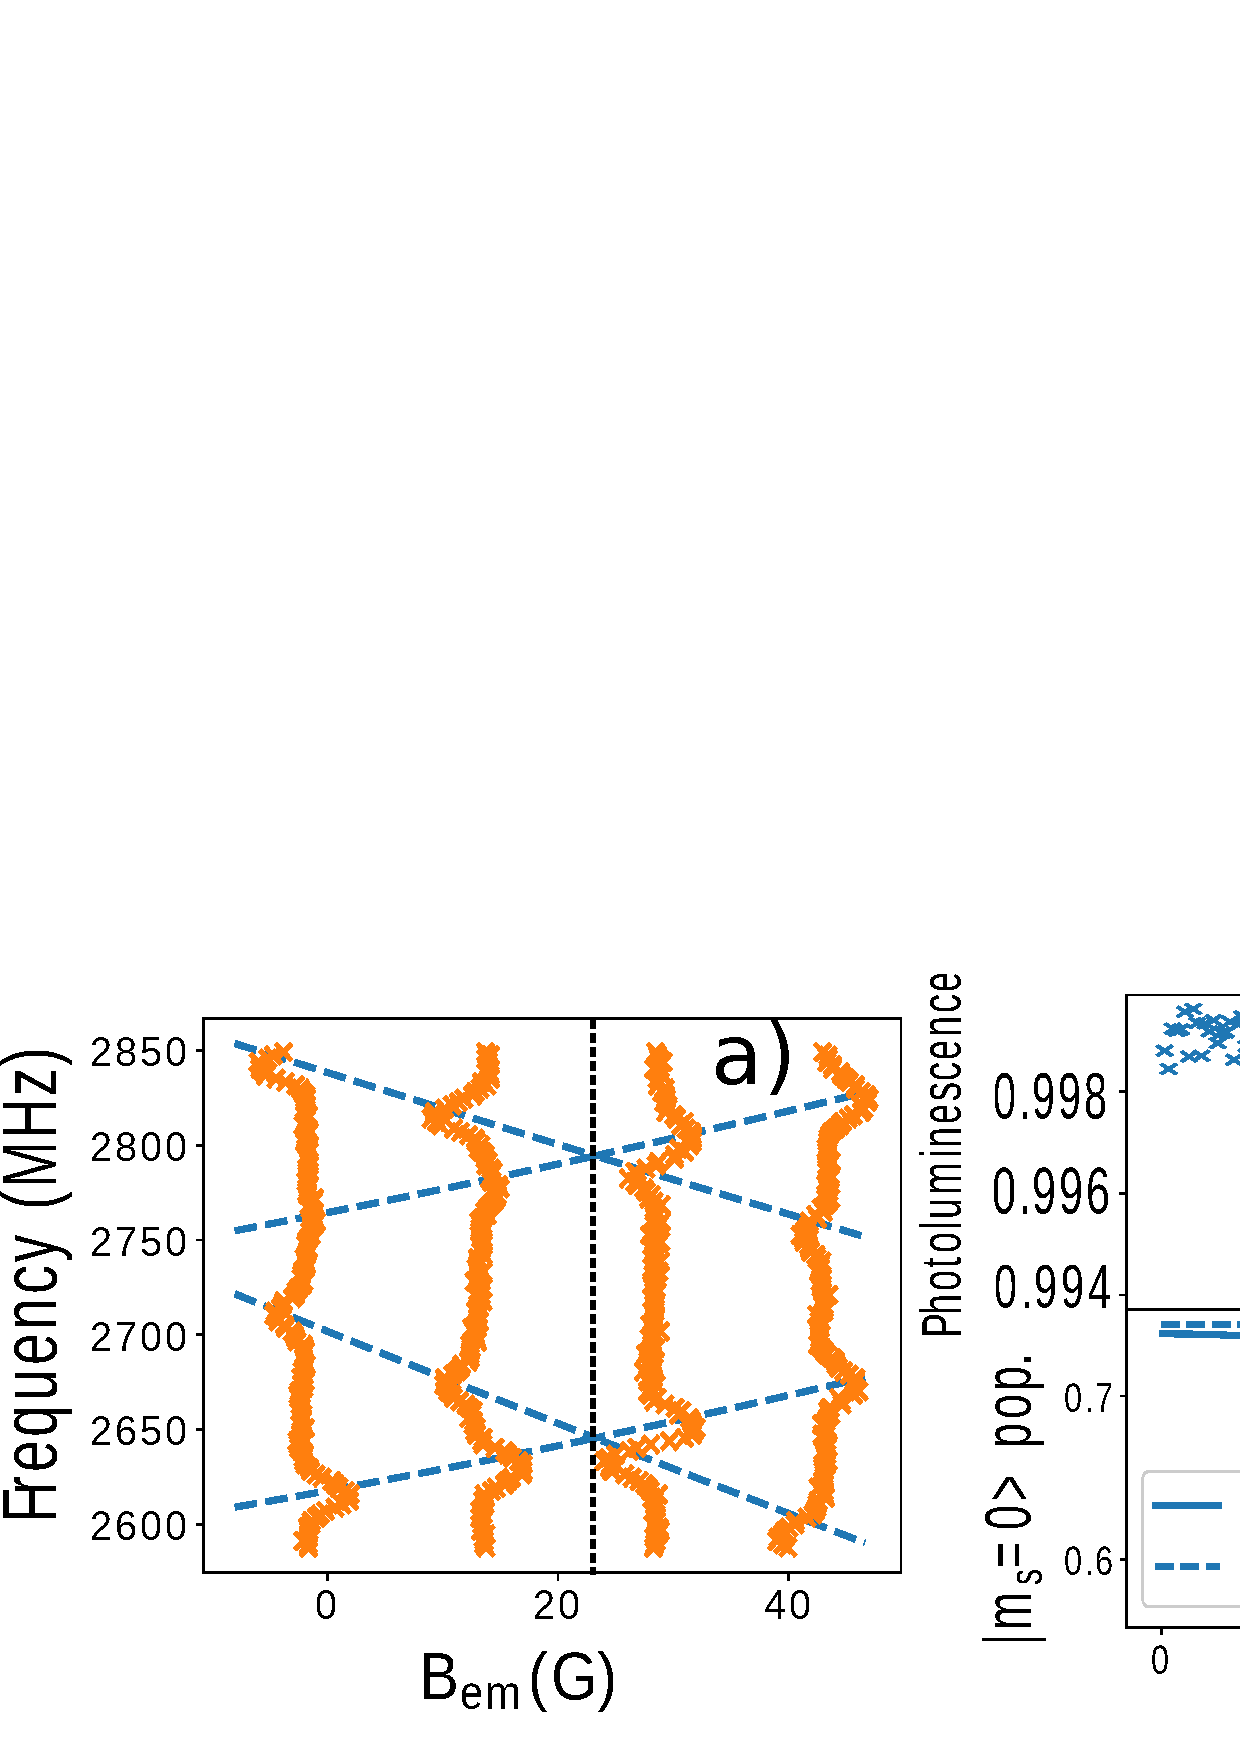
\includegraphics{CR_meca_22}}
  \caption{Mechanical detection of a degeneracy in a [100]$_\perp$ plane. a) Theoretical frequencies for the four $\ket{0} \to \ket{-1}$ transitions in dashed lines and mechanical ESR spectra vertically. b) Photoluminescence of the NV centers as a function of the scanning magnetic field (blue crosses) and gaussian fit (orange line). c) Simulated population in $\ket{m_s=0}$ for the stationary state with (plain) or without (dashed) taking into account the decrease of the T$_1$ induced by the cross-relaxations.
  d) Reflected signal off the diamond as a function of the scanning magnetic field (blue crosses) and double gaussian fit (orange line) e) Simulated torque applied by the spins on the diamond, with (plain) or without(dashed) taking into account the cross-relaxations.}
	\label{CR_22}
\end{figure}

Similarly to Fig. 3 of the main text, we managed to mechanically detect another type of NV-NV resonance. Fig. \ref{CR_22}a) shows the theoretical frequencies of the $\ket{0} \to \ket{-1}$ transitions for all four classes of NV and ESR spectra measured through the reflected laser light off the diamond for various magnetic field values. Unlike The experiment of the main text, this time all four classes of NV are at resonance with another class at B=23 G, telling us that we are crossing a [100]$_\perp$ plane instead of a [110]$_\perp$ one.

Fig. \ref{CR_22}b) shows the recorded photoluminescence of the NV centers during the magnetic field scan. As previously, we see a drop in the luminosity when the resonance occurs, that we fitted with a gaussian. The drop is slightly more pronounced in this case since all classes are depolarized, instead of only two in the previous experiment. This behavior is predicted by the simulation of the $\ket{m_s=0}$ population in the stationary state in Fig. \ref{CR_22}c).

Fig. \ref{CR_22}d) shows the signal of the reflected laser off the diamond, allowing us to measure angular displacement. This time we see a clear difference with the experiment of the main text, instead of a single drop centered on the resonance, we see two bumps on both sides of the resonance, fitted with two gaussians.
This is in accordance with the simulated torque in Fig. \ref{CR_22}e) where we can see a dispersive profile with an almost zero torque at the resonance. The reason we do not observe a change of sign in the experiment (with two positive bumps instead of a positive and a negative one) might be because of the strong non-linearity of our detection : if the signal initially correspond to a dark spot of the speckle, then a change in the motion of the diamond can only result in an increased signal. We also note a drop both in the predicted torque amplitude, and in the signal-to-noise ratio  of the angular measurement compared to the single degeneracy case, implying a weaker effect.

Our physical interpretation of the angular signal we observe, as well as the dispersive profile of the torque is that in this case, for symmetry reason, the magnetic torque generated by the four classes of NV is not modified when we are exactly at resonance, since all four classes are affected identically. What happens when being near, but not at, resonance is that the classes will not be identically depolarized : looking at Fig. \ref{CR_22}a), we can see that the two classes of higher frequency are always slightly closer to each other than the two classes of lower frequency (we can see the slope of the frequencies being a bit smaller for the two upper classes), resulting in a bit more depolarization for these two classes, except when they are exactly at resonance. This interpretation accounts both for the overall shape of the responses, and the comparatively weakness of the phenomenon.


\section{Simulation details}
\label{Simu}
In this part we will discuss the method used to simulate the average torque as well as the $\ket{m_s=0}$ population of the stationary state. The numerical solving of the master equations was performed thanks to the Quantum Toolbox in Python (QuTiP) \citep{qutip1} \citep{qutip2}.

In order to describe the dynamics of our spin ensemble, besides the spin Hamiltonian described in the first part, we introduce the incoherent optical pumping through the jump operators $\mathcal{L}_+ = \Gamma_l \ket{0}\bra{+1} $ and $\mathcal{L}_- = \Gamma_l \ket{0}\bra{-1} $, where $\Gamma_l \approx (2\pi) 10$kHz is the polarizing rate due to the laser.

We also introduce the usual T$_1$ jump operators $\mathcal{L}_i^j= \frac{1}{T_1}\ket{i}\bra{j}$ where $\ket{i,j}$=$\ket{0, \pm 1}$

In order to describe the T$_1$ modification induced by the cross-relaxations, we use a phenomenological model where each class as its own T$_1^i$ (i from 1 to 4) that depends on the energy levels of the other classes with the formula :
\begin{equation*}
\frac{1}{T_1^i}=\frac{1}{T_1^0}+\sum_{j \neq i} \frac{1}{T_1^{dd}}e^{-\frac{(\nu_i-\nu_j)^2}{2(\sigma^{dd})^2}},
\end{equation*}
where $\nu_i$ and $\nu_j$ are the transition frequencies of the classes i and j (we are arbitrarily considering the $\ket{0} \to \ket{-1}$ transition here, since the resonance condition is the same for both transitions at the magnetic fields we are working at. This would not always be true for magnetic fields greater than 592 G\citep{van_oort_cross-relaxation_1989}). 

$\sigma^{dd} = 6$ MHz is the the dipolar interaction width, which we measured to be similar to the inhomogeneous broadening.

$T_1^0=1.03$ ms and $T_1^{dd}=0.38$ ms were chosen to match the T$_1$ measured in Fig. 1 of the main text. We only focus on the T$_1$ without degeneracy and the one with a single degeneracy since our experiments will not have more than two classes at resonance at once. Our model is probably not suited to deal with triple our quadruple resonances.

Finally, according to previous measurements \citep{choi_depolarization_2017}, only the $\ket{0}\bra{\pm1}$ and $\ket{\pm1}\bra{0}$ (corresponding to a single quantum exchange in the dipole-dipole interaction) operators are modified by the cross-relaxations.

With this model in consideration, we can numerically solve the master equation and get the density matrix in the stationary state $\rho_s$. With $\rho_s$ we can directly obtain the $\ket{m_s=0}$ population, corresponding experimentally to the photoluminescence.

As for the torque, we use a semi-classical formula :
\begin{equation*}
\mathbf \Gamma = N_0 \gamma_e \langle\hat{\mathbf S}\rangle \times \mathbf B,
\end{equation*}
where $N_0 \approx 10^9$ is an estimate of the number of spins in our sample based on the average size and NV density of our diamonds, $\gamma_e$ is the gyromagnetic ratio of the electron and $\langle\hat{\mathbf S}\rangle =\mathrm{Tr}(\rho_s \mathbf{\hat S})$ is the averaged spin vector in the stationary sate, averaged again on the four possible orientations of NV.
This formula assumes that the spin dynamics is faster than the dynamics of the motion of the diamond, which is the case in our experiments.

In our plots in Fig. \ref{CR_22} and Fig. 3 of the main ext, we only represent one spatial component (e.g. $\Gamma_x$) of the torque, but the three components behave similarly.
\bibliography{trap}

\end{document}
